\documentclass[12pt]{article}
\usepackage{color}
\usepackage[usenames,dvipsnames,svgnames,table]{xcolor}
\definecolor{dark-red}{rgb}{0.7,0.1,0.1} 
\definecolor{dark-blue}{rgb}{0,0,0.7} 
\usepackage[linkcolor=dark-red,
            colorlinks=true,
            urlcolor=dark-blue,
            pdfstartview={XYZ null null 1.00},
            pdfauthor={Gaurav Sood, gsood07@gmail.com},
            citecolor=dark-red,
            bookmarks=false,
            pdfborder={0 0 0},
            pdftitle={Precise Numerical Summaries}]{hyperref}
            
\usepackage{amsfonts,amssymb,amsbsy,amsmath,amsxtra}

\usepackage[letterspace=500]{microtype}
\usepackage{libertine}
\usepackage[T1]{fontenc}

\usepackage{indentfirst}
\usepackage{setspace} % To set line spacing
\usepackage{multirow}

\usepackage{verbatim}

\usepackage[multiple]{footmisc}
\usepackage{fancyvrb}

\usepackage{longtable}

\usepackage[margin=1in]{geometry}
\usepackage{graphicx}

\raggedright
\parindent=1.5em % <- or whatever indent you want

\usepackage{natbib}
\usepackage{url}
\begin{comment}

\raggedright
\parindent=1.5em % <- or whatever indent you want

\begin{comment}

setwd(paste0(basedir, "quant-discipline/ms"))
tools::texi2dvi("quant.tex", pdf=TRUE, clean=TRUE) 
setwd(basedir)

\end{comment}

\begin{document}
\title{\vspace{-.5cm}\normalsize{\textbf{By the Numbers: Toward More Precise Numerical Summaries of Results}}\footnote{The idiom, ``Do as I say, not as I do,'' aptly summarizes, both, our own limitations in following what we think is good advice, and our hope that our limitations do not detract the readers from the message. Note also that the examples of crude summaries presented here were chosen not because we thought that the passages were particularly notorious but because they were handy. We thank Andrew Gelman, Don Green, Kabir Khanna, Brendan Nyhan, and Daniel Stone for useful comments. The data and the scripts behind the analysis presented here can be downloaded at: \url{http://github.com/soodoku/quant-discipline/}}\vspace{.5cm}}
\author{\normalsize{Gaurav Sood}\footnote{Gaurav is a data scientist. He can be reached at: \href{mailto:gsood07@gmail.com}{\small{gsood07@gmail.com}}} \and \normalsize{Andy Guess}\footnote{Andy is a Moore Data Science Fellow at NYU. He can be reached at: \href{mailto:aguess@gmail.com}{\small{aguess@gmail.com}}}}
\date{\vspace{.5cm}\normalsize{\today}}
\maketitle
\doublespacing

\clearpage
Unlike the natural sciences, there are few true zeros in the social sciences \citep[p. 960,][]{gelman2011causality}. All sorts of variables are often weakly related to each other. And however lightly the social scientists, exogenous events, or other actors intervene, effects of those interventions are rarely precisely zero. When there are few true zeros, categorical statements like `two variables are significantly related', or `the intervention had a significant effect', convey limited information---about sample size and luck (and manufactured luck). Yet these kinds of statements are the norm in abstracts of the top political science journal, the American Political Science Review (APSR).  As we show later, only 10\% of the empirical articles in recent volumes of APSR have abstracts with precise quantitative statements. The comparable number for American Economic Review (AER) is 35\%.

Informal inspection also suggests that crude descriptions are common in other sections of social science articles, aside from being exceedingly frequent in the social science vernacular. (We would like to quantify both.) Studies are often summarized as ``the study shows this broad phenomenon exists.''\footnote{For instance, \citet{pasek2015} write, ``Moreover, much past research shows that guessing is often biased''} For instance, a study on selective exposure summarizes findings of some studies as follows: ``Several studies document a correspondence between people's beliefs and the information to which they are exposed.''\footnote{The excerpt is from \citet{stroud2008}.} Surprisingly, comparison of results often enough also takes the same form. For instance, a study on motivated learning contextualizes the results as follows: ``Our finding is consistent with other research showing that even when people agree on factual information, they often still interpret the information in a motivated manner.''\footnote{The excerpt is taken from \citet{khanna2015}.} The phrase `finding is consistent with' yields nearly 300,000 results on Google Scholar. And informal inspection suggests that `consistent' covers a surprisingly large range of effect sizes, and measures.    

None of this is to say that the decision to use imprecise summaries instead of more precise numerical summaries is made without deliberation. Undoubtedly, some people resort to categorical statements because they think cruder summaries are a more effective way to communicate. Some evidence suggests as much. A survey of undergraduate and graduate students found that 77\% of the students thought that people preferred to receive verbal expressions of uncertainly over numerical in their everyday life \citep{wallsten1993preferences}. (Though, the paper also notes that 85\% of the students felt comfortable switching to another mode if they thought the other mode suited the needs better.) 

Our hunch, however, is that the most common form of crude summaries in scientific communication---categorical statements around statistical significance---arise as a natural consequence of scientists thinking in terms of the Null Hypothesis Statistical Testing (NHST) framework, which in turn is likely underpinned by a Popperian understanding of science \citep{gelman2013philosophy}. Hypotheses in the form of crude categorical statements like, `X will be positively associated with Y,' are exceedingly frequent. And they reflect an understanding of science that is driven by `falsification' than better measurement. 

Whatever the root cause, the use of crude summaries likely leads to serious problems. Firstly, crude summarizations risk misinterpretation. Partly because the mapping between verbal phrases and numerical ranges varies between communicators and recipients \citep{capriotti2011miscommunication}, there is a high degree of variability in how people map verbal expressions to numbers \citep{beyth1982probable, bocklisch2010role, brun1988verbal, simpson1944specific, simpson1963stability}. For instance, \citet{beyth1982probable} elicited numerical mappings of 30 verbal expressions on a 100 point scale, and found that the average inter-quartile range of the mapping for a phrase was 14.4. Analogous numbers---standard deviations of the mapping---from \citet{brun1988verbal}, based on 27 phrases, and \citet{bocklisch2010role}, based on 13 phrases, were 14.2\% (translated from a 0--6 scale) and 11.15 respectively. Relatedly, survey researchers mapping numerical ranges to verbal phrases in a way that minimizes misclassification error, find that even optimal linear boundaries yield a 28\% error rate \citep{elsaesser2013much} (see also \citet{bocklisch2010role}). 

Not only are the mappings variable, mappings also vary systematically as a function of both, phrases, and characteristics of the recipient. Prominently, numerical mappings of verbal phrases about infrequent events, for e.g., seldom, rarely, uncommon, tend to be much less reliable \citep{wallsten1986base}. Interpretation of vague verbal summaries is also subject to cognitive errors. More vague a statement, lower the information, but also greater the opportunity to fill in the specifics. And it is plausible, nay likely, that people don't resist the opportunity to impute. And when imputing, often use common cognitive shortcuts like overweighting accessible information, and interpreting things in a way that confirm their prior beliefs \citep{nickerson1998confirmation, tomz2009electoral, brun1988verbal, wright1994much}.

Use of such cognitive shortcuts often leads to systematic biases in inference. For instance, confirmation bias, in the extremum, means that people read an uninformative vague statement as evidence that their prior is correct. It follows that on reading such a statement, people walk away with yet greater certainty about their priors.  For instance, a person who believes that a law allowing concealed carry increases gun crime by 20\% on reading a study summary that `the study shows that law allowing concealed carry increases gun crime' may optimistically conclude that the study shows that allowing concealed carry increases gun crime by 20\%. The same person reading a summary that `the study shows that law allowing concealed carry decreases gun crime' may optimistically conclude that the decline is at worst tepid. 

Lastly, crude summaries may lead to another erroneous imputation because of how people understand everyday use of language. For instance, a person with flat priors about selective exposure on reading a study summary that ``people engage in selective exposure'' may interpret it reasonably as ``most people read news stories from sources that they think are aligned with their party.'' A more precise numerical statement of the sort that gives the proportion of news stories consumed from ideologically congenial sources preempts the risk of such misinterpretation. 

Besides misinterpretations of topical effect sizes, crude summarizations also risk conveying incorrect ways of thinking about science---as falsification or crude directional claims, than as an effort of getting better---less biased and more precise---estimates of actual quantities of interest. Presenting more precise estimates may instill in readers a better appreciation of the point that Don Green made in an interview in the aftermath of the fake data scandal, ``That's what makes the study interesting. Everybody knows that there's some degree of truth in these propositions, and the reason you do an experiment is you want to measure the quantity.''\footnote{``An Interview With Donald Green, the Co-Author of the Faked Gay-Marriage Study.'' Jesse Singhal. NY Mag. Published on May 21, 2015. \href{http://nymag.com/scienceofus/2015/05/co-author-of-the-faked-study-speaks-out.html}{http://nymag.com/scienceofus/2015/05/co-author-of-the-faked-study-speaks-out.html}} Making more precise numerical statements may also improve how we understand the results of studies. And over the longer term, by making us think more carefully about our priors, precise numerical summaries may improve how we think about science, and interpret scientific results. For instance, presenting precise numerical summaries in the abstracts may help us more quickly filter studies in which results are ``too big.''\footnote{\href{http://www.washingtonpost.com/blogs/monkey-cage/wp/2014/12/19/pushing-at-an-open-door-when-can-personal-stories-change-minds-on-gay-rights/}{Pushing at an open door: When can personal stories change minds on gay rights?} Andrew Gelman. Monkey Cage. The Washington Post. Published on December 19, 2014.}

With that preface, we move to empirically examine the frequency of crude judgments in abstracts that traditionally carry the summary of the results of the study in the social sciences.

\section*{How Common Are Precise Numerical Summaries in Abstracts?}
\label{sec:sum}
To assess how common crude judgments are vis-\`{a}-vis more precise numerical statements, we coded 310 abstracts--- 117 APSR, 93 American Economic Research Papers and Proceedings (AER P \& P), and another 100 from other American Economic Research (AER) journals. We subset on empirical papers--- 66 (AER), 68 (AER P \& P), 81 (APSR).

What we mean by precise numerical statements deserves careful attention. Precision is on a continuum, with statements going from very imprecise to very precise. But for clarity and convenience, our coding scheme captures only one end of the scale. We code statements that take the following form as precise: `A\% change in X caused a B\% change in Y' or `the intervention caused B\% change in Y.' Some examples of statements we code as precise: ``The average proportion of ``no'' votes is about 40\% higher for applicants from (the former) Yugoslavia and Turkey,'' ``I find that a one-percentage-point increase in the personal vote received by a gubernatorial candidate increases the vote share of their party's secretary of state and attorney general candidates by 0.1 to 0.2 percentage points.'' etc. And we code any other statement as imprecise. For instance, we code the following statements as imprecise: ``increasing numbers of armed military troops are associated with reduced battlefield deaths'', ``We find support for these arguments using original data from Uganda.'' etc. 

\begin{figure}[htbp]
\centering
\caption{Proportion of Precise Numerical Statements in Abstracts of Empirical Papers in the APSR, AER, and the AER P \& P}
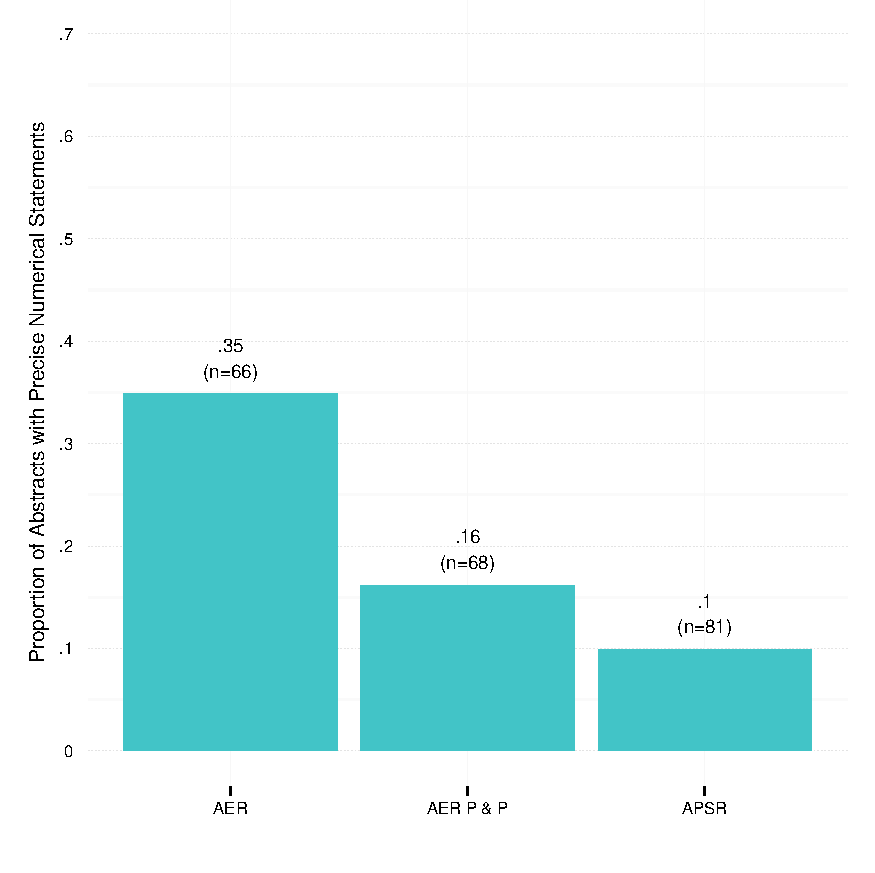
\includegraphics[scale=.75]{../figs/apsr_aer.pdf}
\label{fig:summary}
\end{figure}

Only about 10\% of the empirical articles in recent volumes of APSR have abstracts with precise quantitative statements, similar to the percentage for AER P \& P. The comparable number for AER is 35\% (see Figure~\ref{fig:summary}). None of the numbers are appealing, but the numbers for APSR are particularly galling. 

In toto, by shedding light on the problem, it is our hope that the article stimulates discussion about social scientific writing. And increases efforts to address likely the root cause of a particularly common crude description---categorical statements around statistical significance. 

\clearpage
\bibliographystyle{apsr}
\bibliography{quantbib}


\end{document}
